\documentclass[runningheads]{llncs}
\usepackage[T1]{fontenc}
\usepackage{lmodern}
\usepackage{microtype}
\usepackage[hidelinks]{hyperref}
\usepackage{pgfplots}
\usepackage{ragged2e} 
\pgfplotsset{compat=1.17}

\renewcommand{\UrlFont}{\small\ttfamily} 

\sloppy

\titlerunning{Deep Learning Approaches for Alzheimer’s Classification}
\title{Deep Learning Approaches for Alzheimer’s Disease Classification Using MRI Images}
\author{Rareș-Andrei Filip\inst{1} \and Dragoș Ilieș\inst{1}}
\institute{
Faculty of Economics and Business Administration (FSEGA), \\
Babeș-Bolyai University (UBB), Cluj-Napoca, Romania
}

\begin{document}
\maketitle

\begin{abstract}
    % Abstract-ul va fi completat ulterior.
\end{abstract}


\section{Introduction}

Alzheimer's Disease (AD) is a progressive neurodegenerative disorder that affects memory, cognitive function, and daily activities. It is the most common cause of dementia, accounting for approximately 60–80\% of cases globally~\cite{helaly2021}. According to recent statistics, over 50 million people are currently living with AD worldwide, and this number is expected to rise to 152 million by 2050. Early diagnosis of AD is critical to slowing the progression of the disease, enabling timely interventions that improve patients' quality of life.

Magnetic Resonance Imaging (MRI) has become an essential tool for detecting structural brain changes associated with AD. These images reveal subtle differences in brain regions such as the hippocampus and gray matter, which are commonly affected in the early stages of the disease. However, traditional methods for analyzing MRI data rely heavily on manual interpretation and handcrafted feature extraction, which are time-consuming and prone to human error.

The advent of Artificial Intelligence (AI), particularly Deep Learning (DL), has revolutionized medical imaging analysis. Deep learning models, such as Convolutional Neural Networks (CNNs), have demonstrated superior performance in feature extraction and image classification tasks. Techniques like transfer learning and attention mechanisms have further improved diagnostic accuracy, particularly in the presence of limited annotated datasets.

Despite these advancements, challenges remain:
\begin{itemize}
    \item How can deep learning models achieve robust classification of Alzheimer's and non-Alzheimer's cases using MRI scans?
    \item What are the limitations of existing approaches, and how can they be addressed?
    \item What practical value can these models provide to clinicians for supporting early diagnosis in real-world environments?
\end{itemize}

This study contributes to addressing these challenges by conducting a systematic comparison of Machine Learning (ML) and Deep Learning (DL) techniques. The focus is on leveraging transfer learning, attention mechanisms, and hybrid approaches to develop accurate and computationally efficient models for AD classification.

\section{Related Work}

Several studies have explored the use of machine learning and deep learning techniques for the classification of Alzheimer's Disease using MRI data.

Helaly et al.~\cite{helaly2021} applied transfer learning using pre-trained CNN models, such as VGG19, to classify MRI scans into multiple AD stages. Their work demonstrated the effectiveness of transfer learning in mitigating overfitting when datasets are limited. However, their approach did not explore attention mechanisms, which have been shown to improve feature localization.

Nasir et al.~\cite{nasir2021} proposed an ensemble learning approach by combining multiple CNN architectures. Their method achieved an accuracy of 90\% using majority voting to reduce model variance. While effective, ensemble models often require higher computational resources, which can limit their practicality in clinical settings.

Pandiyaraju et al.~\cite{pandiyaraju2022} introduced a dual-attention-aware CNN architecture to improve classification accuracy. By focusing on critical brain regions like the hippocampus, their model achieved state-of-the-art results with an accuracy of 99.1\%. This highlights the potential of attention mechanisms in enhancing the performance of deep learning models.

Jo et al.~\cite{jo2021} explored multimodal approaches by combining MRI and PET data. Their use of stacked autoencoders and CNNs achieved accuracies exceeding 98\%, demonstrating the benefits of integrating complementary imaging modalities for improved diagnostic performance.

Hybrid approaches combining machine learning and deep learning techniques have also been investigated. Khvostikov et al.~\cite{khvostikov2022} utilized structural and diffusion imaging data with feature extraction techniques to improve diagnostic accuracy. However, their work relied heavily on manual feature engineering, which can be time-consuming and prone to errors.

In summary, while existing methods have achieved high accuracy, they face limitations such as high computational demands, reliance on large annotated datasets, and lack of integration into real-world clinical workflows. This study builds upon these contributions by exploring transfer learning, attention mechanisms, and hybrid frameworks to develop a robust and efficient solution for AD classification.

\section{Dataset Description}

The Alzheimer MRI Disease Classification dataset~\cite{dataset_source} provides a structured collection of Magnetic Resonance Imaging (MRI) brain scans, categorized into four classes based on varying stages of cognitive impairment. This dataset is highly appropriate for our research as it allows for the evaluation of deep learning and machine learning methods in detecting Alzheimer's Disease (AD) across different levels of severity. By including multiple stages of the disease, the dataset facilitates a more comprehensive analysis, addressing both binary classification (Alzheimer's vs. Non-Alzheimer's) and multi-class classification tasks.

The dataset consists of grayscale 2D MRI images that represent structural brain changes associated with AD progression. Such changes are particularly visible in regions like the hippocampus and gray matter, which are critical for detecting early and subtle signs of the disease. The presence of labeled data makes it suitable for supervised learning techniques, and the class imbalance reflects real-world scenarios, further validating the dataset's applicability in clinical practice.

Figure~\ref{fig:sample_images} illustrates sample MRI images from the dataset, showcasing the visual differences across the four classes.

\begin{figure}[htbp]
    \centering
    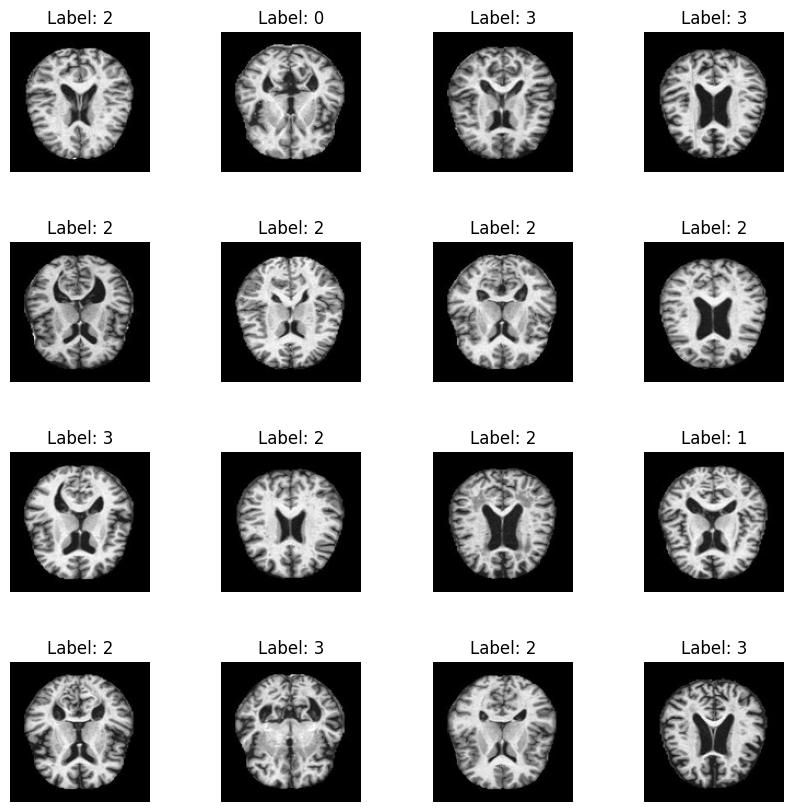
\includegraphics[width=0.8\textwidth]{C:/Users/Dragos/Documents/Deep learning/Alzheimer_Project/sample_image}
    \caption{Sample MRI images from the dataset.}
    \label{fig:sample_images}
\end{figure}

\noindent
\textbf{Legend:}
\begin{itemize}
    \item Label 0: Mild Demented
    \item Label 1: Moderate Demented
    \item Label 2: Non-Demented
    \item Label 3: Very Mild Demented
\end{itemize}

\subsection{Data Preprocessing}
Before training the models, the dataset underwent the following preprocessing steps:
\begin{enumerate}
    \item Resizing: All MRI images were resized to $128 \times 128$ pixels for uniform input dimensions.
    \item Normalization: Pixel values were normalized to the range [0, 1].
    \item Augmentation: To address class imbalance, data augmentation techniques such as horizontal flipping, rotation, and scaling were applied to the underrepresented classes.
\end{enumerate}

\subsection{Class Distribution}
The dataset contains an uneven distribution of images across the four classes, as shown in Table~\ref{tab:class_distribution}. This distribution highlights the class imbalance, with the `Non-Demented` class containing the most samples and the `Moderate Demented` class having the least. To address this imbalance, data augmentation techniques were applied during preprocessing.

\begin{table}[htbp]
    \centering
    \caption{Distribution of Classes in the Alzheimer's MRI Dataset}
    \label{tab:class_distribution}
    \begin{tabular}{|l|c|}
        \hline
        \textbf{Type of Alzheimer’s Disease} & \textbf{Images Count} \\ \hline
        Non Demented                         & 2560                  \\ \hline
        Very Mild Demented                   & 1792                  \\ \hline
        Mild Demented                        & 717                   \\ \hline
        Moderate Demented                    & 52                    \\ \hline
    \end{tabular}
\end{table}

\sloppy
\bibliographystyle{splncs04}
\bibliography{references}

\end{document}
